%
% File acl2019.tex
%
%% Based on the style files for ACL 2018, NAACL 2018/19, which were
%% Based on the style files for ACL-2015, with some improvements
%%  taken from the NAACL-2016 style
%% Based on the style files for ACL-2014, which were, in turn,
%% based on ACL-2013, ACL-2012, ACL-2011, ACL-2010, ACL-IJCNLP-2009,
%% EACL-2009, IJCNLP-2008...
%% Based on the style files for EACL 2006 by 
%%e.agirre@ehu.es or Sergi.Balari@uab.es
%% and that of ACL 08 by Joakim Nivre and Noah Smith

\documentclass[11pt,a4paper]{article}
\usepackage[hyperref]{acl2019}
\usepackage{times}
\usepackage{latexsym}
\usepackage{graphicx}
\usepackage{wrapfig}

\usepackage{url}

\aclfinalcopy % Uncomment this line for the final submission
%\def\aclpaperid{***} %  Enter the acl Paper ID here

%\setlength\titlebox{5cm}
% You can expand the titlebox if you need extra space
% to show all the authors. Please do not make the titlebox
% smaller than 5cm (the original size); we will check this
% in the camera-ready version and ask you to change it back.

\newcommand\BibTeX{B\textsc{ib}\TeX}

\title{ NLP report}

\author{Author \\
  Aiden Deng / ad1821@ic.ac.uk \\
  Jinli Yao / jy4917@ic.ac.uk \\
  Yining Kang / fk521@ic.ac.uk \\
  Github Reference: \href{https://github.com/kangyining/NLP_2022}{Link}  
 \\}

\date{}

\begin{document}
\maketitle
\section{Introduction}
In this paper, we construct an NLP model which gives binary classification towards usage of Patronizing and Condescending Language(PCL) on various media posts. PCL is used when the speaker/author uses a superior attitude towards others or describes their situation in a benevolent way. PCL itself is often implicit and unconscious, which makes it extremely hard and ambiguous to detect. On the contrary, its effect can be quite harmful and can boost the existing discrimination. Therefore, we believe identifying the PCL is a crucial feature for modern media.

We use the \textit{Don't Patronize Me!}\cite{perez-almendros-etal-2020-dont} dataset provided by the competition organizer, and we first perform analysis on it. In terms of the class labels, we use 0 to indicate a negative sample and 1 to indicate a positive sample. To analyze the data distribution and the correlation between input length and label, we generate the following graph:
\begin{figure}[h]
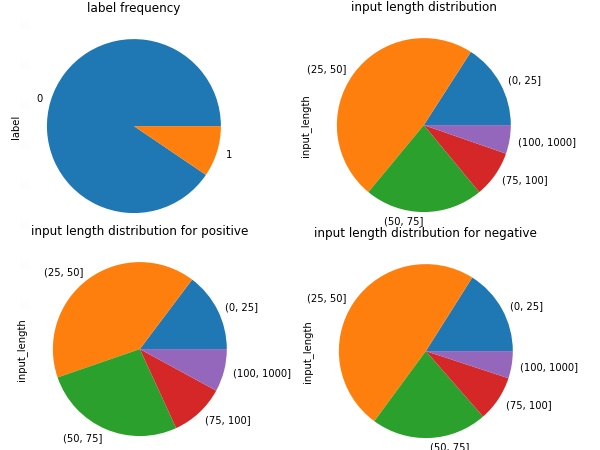
\includegraphics[width=0.45\textwidth, height=150pt]{figures/frequency.jpg}
\end{figure}

We can see that from the first graph, the data is heavily skewed and there are many more negative examples than positive examples (in fact, the number of negative samples is roughly 10 times the number of positive samples). From the rest of the graphs, we can see that although there is some correlation between the input length and the final label, the overall distribution remains similar for both the positive and negative examples. Using Point-Biserial Correlation for quantitative analysis, we get a positive correlation of around 0.053 and a super small p-value ($<1.5E(-6)$). We then conclude that there is a very weak positive correlation between the input length and final label.

Furthermore, we think the task is quite subjective and hard. The subjectivity can be inferred directly from the definition of the PCL: It is often "involuntary" and "unconscious", and the author may have a benign purpose and means no harm to the readers at all. But from the readers' perspective, the media post could seem to express superiority and thus unacceptable. Let's also check one example. "Egypt billionare offers to buy Mediterranean island for refugees" is one of the samples that was labelled as positive, although we think the sentence is rather objective and won't lead to a feeling of PCL at all. We believe the task is also hard, coming from both its subjectivity and the non-explicitness of indicative words. We generate two word count plots (the larger version on GitHub).
\begin{figure}[h]
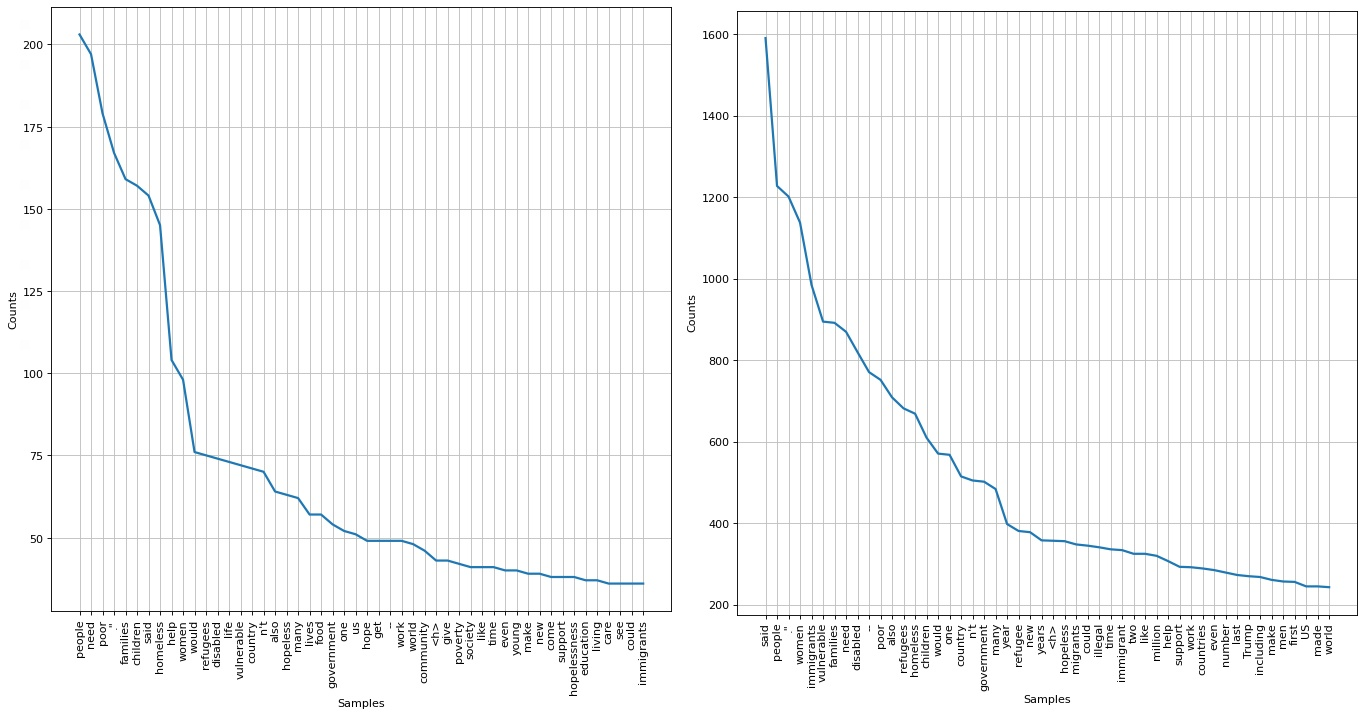
\includegraphics[width=0.45\textwidth, height=75pt]{figures/word_count_plot.jpg}
\end{figure}
From the plots, we can see quite a few common words are just "neutral". For example, it is obvious that "people", "need" or "said" are just neutral words and don't have any "superior" meaning for sure. For this task, we cannot only rely on the meaning of single words, and need lots of contexts for semantic analysis, which makes the entire task hard.
\section{Modelling} 
\subsection{Data Pre-process}
The first thing we did was data pre-processing. We found that the dataset was clean. In addition, punctuation and stop words are semantically meaningful. Therefore, we only changed the characters of the whole dataset to lowercase.

However, the dataset is extremely unbalanced in terms of labels which is shown in the Introduction. So, we use a weighted negative sampling to sample negative labels.

For the Tokenizer method, we use AutoTokenizer from HuggingFace library. We use byte-level BPE for RoBERTa and punctuation splitting and wordpiece for DeBERTa. The max-length parameter of the Tokenizer is in the range of 1-512. The smaller the parameter, the less time cost in training. However, if the maximum length is exceeded, some data will be intercepted and the information may be lost. Meanwhile, we have enough computing power. Therefore, we use 512 as the parameter.

\subsection{Hyperparameter Searching}
We first searched on the learning rate of RoBERTa-base with CLS pooler as the output layer\cite{liu2019roberta}. We refer to the original paper for the initial value: 1e-5 and test some other possible candidates. In terms of the batch size, we found out that the performance kept increasing as we increased the batch size. Due to GPU video memory limitations, we can only choose batch size up to 16. For loss function, since the original dataset is quite unbalanced, we turned to dice loss\cite{li2020dice}. After testing parameters through 0.3, 0.5, 0.7, and 0.5 produces the best result. We also tried a few weight sampling algorithms. Check tables below for each hyperparameter tuning process (Note that we implemented early stopping, and the epoch shown below is the epoch before the early stop was triggered. Also, we used 12 as the random seed, and we use the official validation, test set as our validation set, test set, separately.):
Some abbreviations: ep = epoch, pr = precision, re = recall, AD = all training set, 3N: 3 - 3 * positive samples size as total size, N: sampling without replacement, Y: sampling with replacement).

\begin{table}[h!]
\begin{tabular}{lllll}
loss f  & ep & pr     & re     & F1     \\
BCE     & 3  & 0      & 0      & 0      \\
DL(0.3) & 3  & 0.4943 & 0.6482 & 0.5609 \\
DL(0.5) & 7  & 0.5607 & 0.6734 & 0.6118 \\
DL(0.7) & 11 & 0.4876 & 0.6935 & 0.5726
\end{tabular}
\caption{tuning loss function, with lr=1e-5}
\end{table}
\begin{table}[h!]
\begin{tabular}{lllll}
lr   & ep & pr     & re     & F1     \\
1e-5 & 7  & 0.5570 & 0.6633 & 0.6055 \\
2e-5 & 4  & 0.5816 & 0.5729 & 0.5722 \\
1e-6 & 7  & 0.5479 & 0.6030 & 0.5742
\end{tabular}
\caption{tuning learning rate, with diceloss(0.5)}
\end{table}
\begin{table}[h!]
\begin{tabular}{lllll}
WS & ep & pr     & re     & F1     \\
AD & 7  & 0.5570 & 0.6633 & 0.6055 \\
3N & 7  & 0.5607 & 0.6734 & 0.6118 \\
3Y & 10 & 0.5397 & 0.6482 & 0.5890
\end{tabular}
\caption{tuning weighted sampling algorithms}
\end{table}

\subsection{Model Selection}
We choose the final model by first tuning them on the training set with different hyperparameters, and then collecting and comparing their performance on the test set. Check the table below for a comparison. Note, we use dice loss(0.5) for loss function, 3N for weighted sampling algorithm, 1e-5 learning rate for RoBERTa-base and 5e-6 learning rate for the others, batch size 16 for both RoBERTa-base and DeBERTa-v3-base\cite{he2021debertav3}, batch size 8 for RoBERTa-large, and batch size 4 for DeBERTa-v3-large. 
\begin{table}[h!]
\begin{tabular}{lllll}
model            & ep & pr     & re     & F1     \\
RoBERTa-base     & 7  & 0.5013 & 0.6182 & 0.5537 \\
DeBERTa-v3-base  & 12 & 0.5337 & 0.6751 & 0.5961 \\
RoBERTa-large    & 12 & 0.5162 & 0.6530 & 0.5766 \\
DeBERTa-v3-large & 10 & 0.6129 & 0.5994 & 0.6061
\end{tabular}
\caption{table for model comparison}
\end{table}
\subsection{Improvements}
We have implemented several improvements to the original model. Details of the following points can be extracted from the code repository. First, instead of the last CLS pooler layer, we tried a few different output structures such as the last layer to LSTM and GRU then concatenate with pooler layer (f1 score on test set 0.6161), last 2 CLS (0.5631), CLS + last token (0.5656), and finally chose LSTM+GRU.

Second, we tried to introduce a few other improvements: including EMA(Exponential Moving Average); including adversarial learning(FGM or SMART\cite{2020}, where FGM provides more improvement); we also clamped gradient to avoid destroying the pre-training result; we applied multi-dropout layer to regularize the neural networks. We apply ablation experiments to verify that all points above have a positive effect on the result.

Third, we tried to introduce ensembling with the hard voting classifier to the model including three models in total, which increased the F1 score from 0.628 to 0.646. The first is deberta-v3-large with lstm gru, the second is Bert lastClsSep + MTD + ems + FGM, and the third is Bert lastClsSep + MTD + ems + clamp + R-drop.

Last, we also tried a few other methods, including data-argumentation, back translate(from Google), synonyms exchange(from wordnet), and concluded that none of them increase the performance in the end.
\section{Analysis}
% 哪里比原模型更好
\subsection{different level of patronizing content}
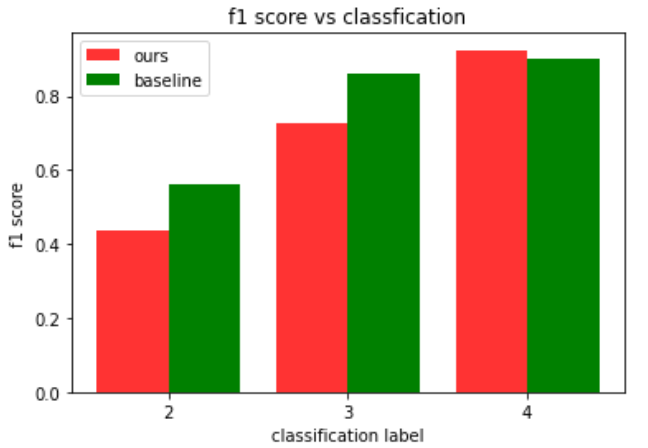
\includegraphics[width=0.45\textwidth, height=120pt]{figures/f1scorevslabel.png}
 The precision, recall and F1 score of RoBERTa baseline on the validation set are 0.3935, 0.653 and 0.4911, respectively. Our model has better data in all three numbers which are 0.5764, 0.6633, 0.6168, respectively. In terms of the higher level of patronizing content, our model did worse (f1 score) than the baseline model on samples labelled with 2 and 3, but did better than the baseline model on samples with label 4. It seems that our model can classify the contents that are highly patronized correctly while performing worse than the baseline model on lowly patronized contents.
%  The current model has 20 more positive results and 326 fewer negative results than the baseline in this file. Since the positive label is minor in data, an increase of 11 true positives leads to a preferable result. Also, more boarder line cases are distinguished. For example, "Hollywood star Leo Di Caprio urges help for reuniting immigrant children with their families." is classified as patronising content as it is not in baseline model.
\\\\
\subsection{input length impact on model performance}
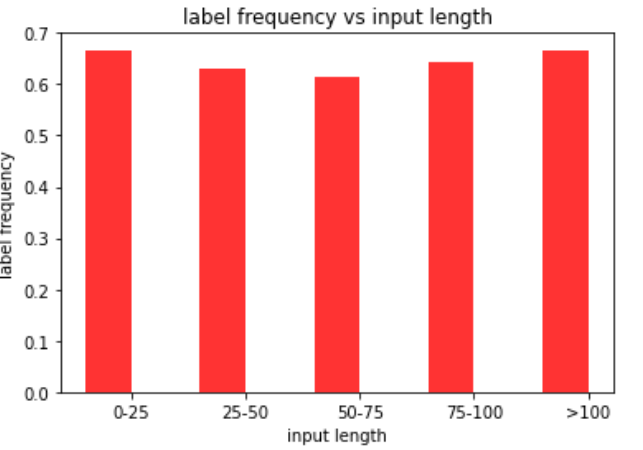
\includegraphics[width=0.4\textwidth, height=70pt]{figures/inputle.png}

% 长度是否有影响
The length of the input sequence does not have much effect on the performance of the model. On the graph above, we can see that for all input length ranges, the accuracy (correctly predicted positive samples over all positive samples in that range) remains roughly the same, with a bit decrease in 50-75 and 75-100. The difference is pretty small and we think that could be a result of the small sample size.
\subsection{categorical data influence}
% 分类是否有影响
% we also analyse how categorical data influence the performance. 
There are two available label kinds for analysing, keyword and country\textunderscore code. For the keyword, our model succeeds in distinguishing some labels and having high f1 scores. "In-need" has the highest f1 score, which is 0.8101. Meanwhile, the model performs badly at distinguishing "refugee" and "immigrant" labels, which have 0.4545 and 0.4444 in f1 scores, respectively. For the country\textunderscore code, "sg" has 1.0000 as f1 score. On the contrary, "au" and "ca" are particularly low, with 0.3333 and 0.4286, respectively. In terms of the country\textunderscore code label, it has a larger spread in f1 score range than the keyword label. It indicates that country\textunderscore code influences the model relatively more than the other label. However, since there are few outliers, we assume only certain indicative words obviously influence the model predictions of our model.
% However, all other categories' F1 are all around model's F1 and few outliers are acceptable. we can say that categorical data do not influence the performance a lot.
\section{Conclusion and further thoughts}
In this task, our model gets a final f1 score of 0.6470, which is pretty good and outperforms the baseline model a lot. From the results, we can see that extracting and classifying the patronizing contents is a very difficult task, and many patterns need much more input data to be validated. For further studies, we can apply cross-validation to mitigate the validation error caused by the small sample size. We can also gather more positive samples (samples categorized as PCL) and corresponding datasets to pre-train or incremental train the model and improve its performance. 
% 在这个任务中我们取得了F1:0.6470的好成绩,比基线模型有很大的提高。从实验结果可以看出想要提取出Patronizing的句子是个很难的任务很多规律都需要更多的数据去验证。在以后,我们可以使用交叉验证来消除小样本带来的验证误差,寻找更多的正样本并且相关数据集对模型进行预训练或者增量训练来提高模型的performence.
% After completing data pre-process, hyperparameter searching, model selection and improvement, we end up with a model. And the final F1 score is 0.6470. According to analysis, the model has a great improvement on precision than the baseline model. Meanwhile, we find out relevant and irrelevant factors of the model and need more data to support the analysis. If we could do more in the future, the first step would be to collect more PCL content. Currently, we have an unbalanced data set, which leads to a worse result. The more positive results we collect, the more accurate the model will be. Another thing is that if we could start training not only from the content but also from the context, this would be a big accuracy improvement.
\bibliographystyle{acl_natbib}
\newpage
\bibliography{references}

\end{document}
